\chapter{系统设计}
在本章中,我们提出并详细描述我们在\cu 的基础上,构建的用于有效电子表格缺陷检测的技术\wa 。
我们首先介绍\wa 的工作流程,以及它和\cu 的关联性。
之后,我们详细展现\wa 的三个几部有效性属性的单元格聚类精化方法。


\section{\wa 的工作流程}
\begin{figure}[tbp]    
    \centering
    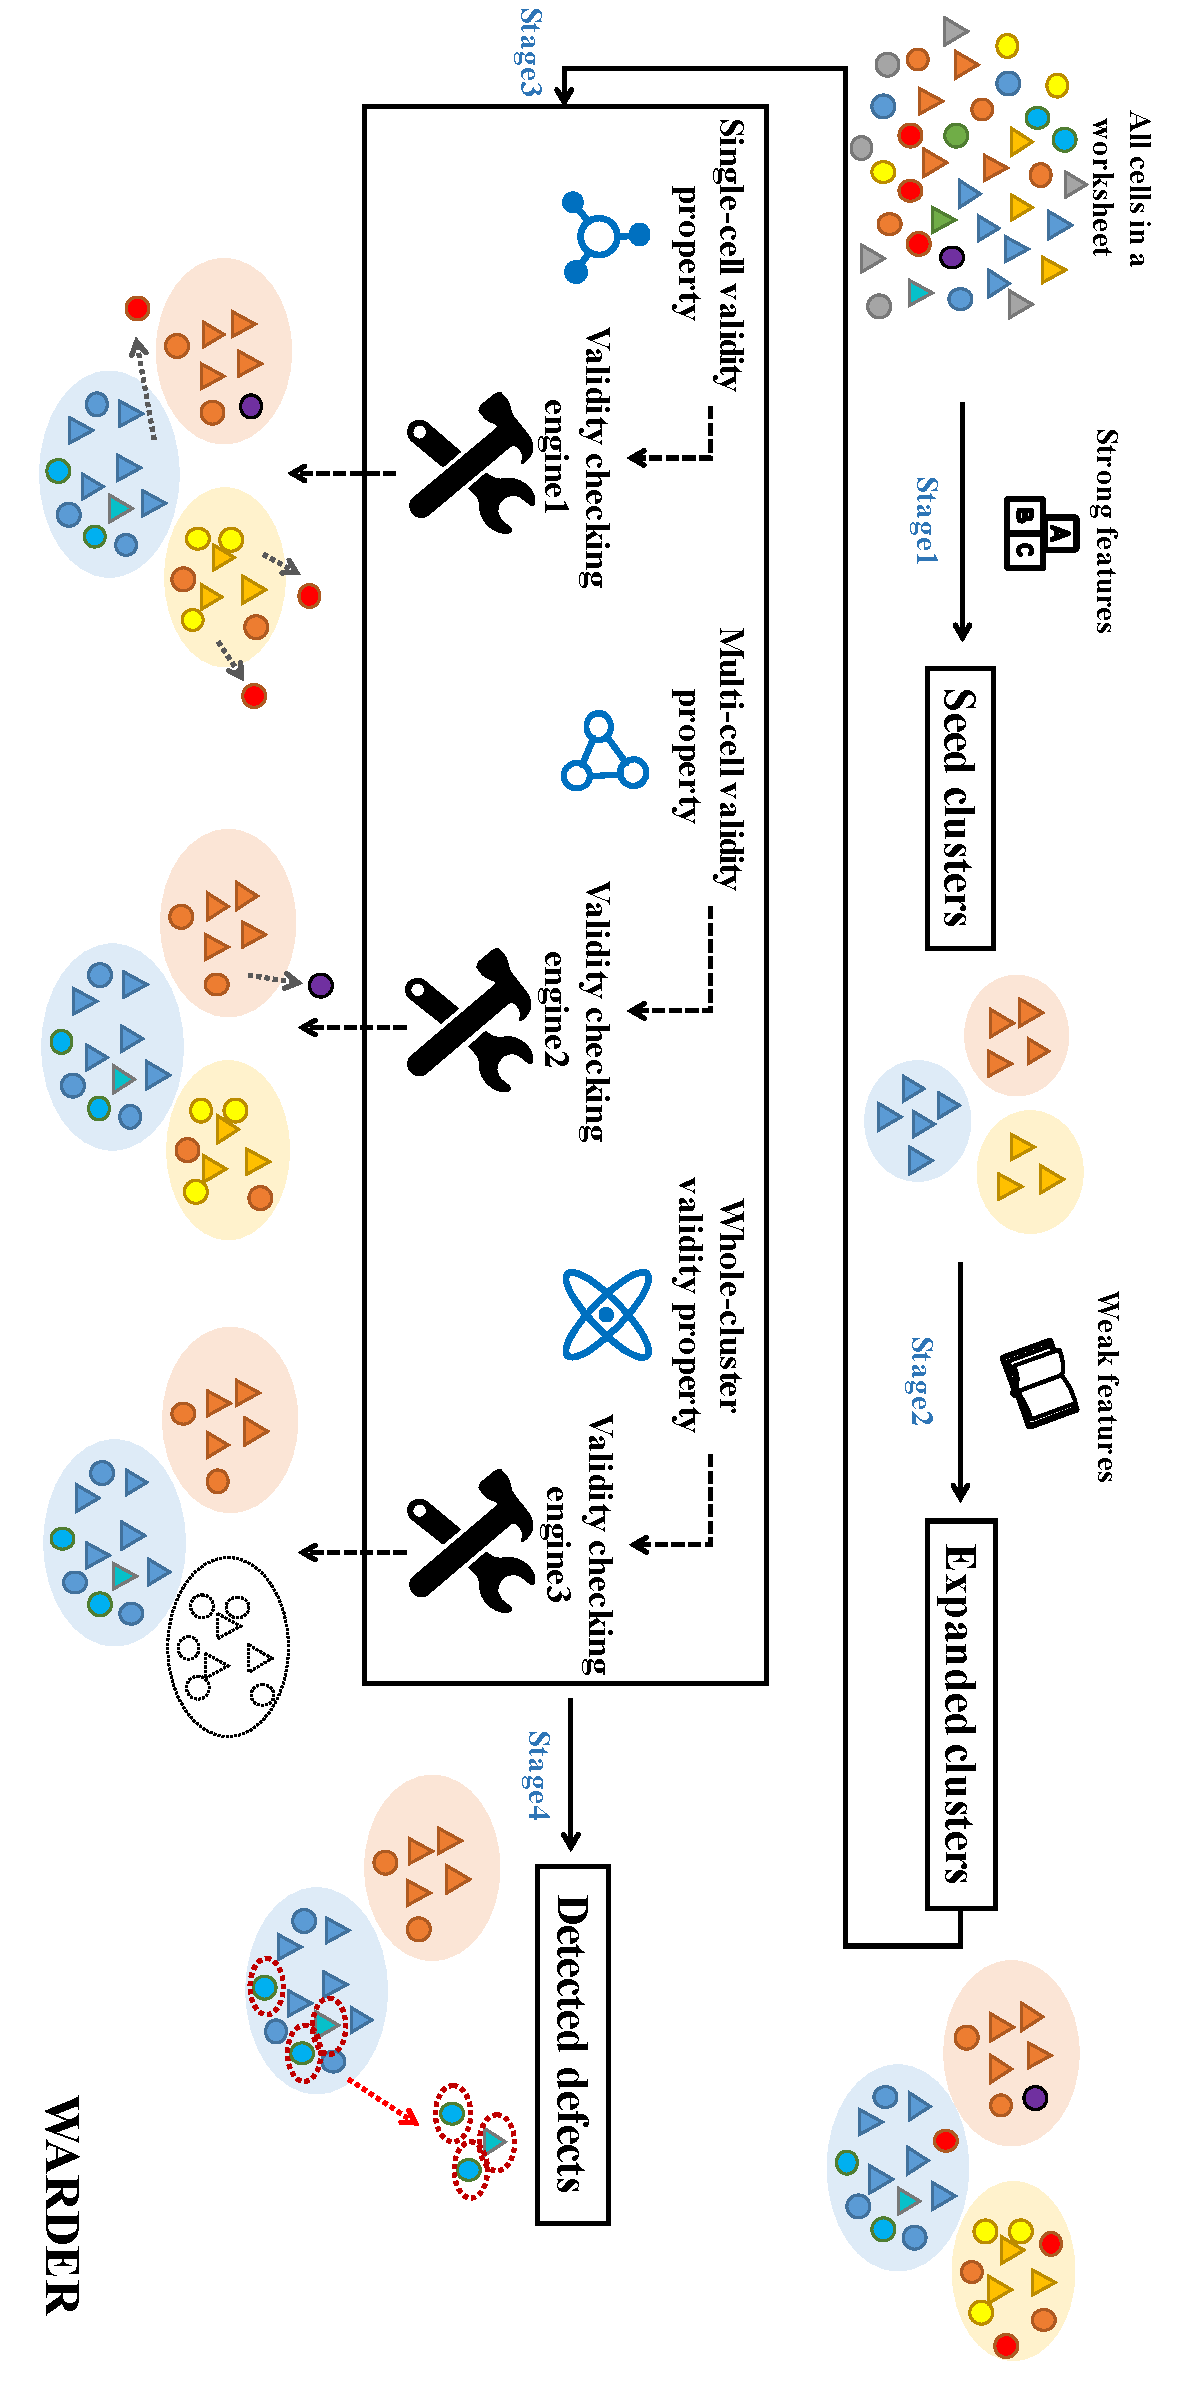
\includegraphics[width=0.7\textwidth]{figure/figure1-copy.pdf}
    \caption{\wa 的工作流程(阶段 3 是相对于它的前身 \cu 的核心贡献点)}
    \label{figure1}
\end{figure}
如图\ref{figure1}所示,\wa ,和\cu 集成在一起,包含四个阶段,在一张工作表里,从对相关单元格的聚类,到在每一个类中检测缺陷。

首先,\wa 使用 \cu 来形成一个种子类的初始集合,这个种子类中的每一个单元格都包含相似的\textit{强特征}(例如单元格公式还和引用关系等)。这个阶段使得每个种子类都包含一个尽可能共同的计算目标。
第二,\wa 使用 \cu 来扩充每个种子类,使用第一阶段剩下没有被分类的单元格作为被扩充的对象,只要这些被扩充的单元格和在第一阶段已经在种子类中的单元格拥有相似的\textit{弱特征}(例如空间关系,字体,颜色和布局等)。第二阶段是的那些在第一阶段被忽视的单元格重新收集起来,这些被忽视的单元格通常由于自身含有有缺陷的公式。
第三,\wa 精化当前的单元格类,通过将那些违反有效性属性的单元格(后面三节会详述这三种属性)从它所属的类中排除出去。第三阶段通过识别不相关的单元格和不合格的单元格类,来提升单元格聚类的质量。
第四,\wa 使用 \cu 来从每个合格的单元格类中识别出异常的单元格,并把这些单元格标记为缺陷,并汇报给用户。第四阶段是在含有共同计算目标的单元格类中检测缺陷,这些有缺陷的单元格要么是丢失了公式,要么是含有和类中其他单元格不一致的公式。

\cu 的优点在于能够将很多单元格扩充到种子类中,从而提升了缺陷检测技术的召回率指标\cite{cheung2016custodes}。
然而,这一扩充过程相对激进,因为它同时也将相当数量的不相关单元格扩充进来,这进一步影响了单元格聚类和缺陷检测的精度指标。
正因如此,这一痛点正是我们的\wa 提出的三个精化方法想要解决的目标,接下来我们详细描述精化过程的细节。


\section{单个单元格自身的有效性精化方法}
\begin{figure}[tbp]
    \centering
    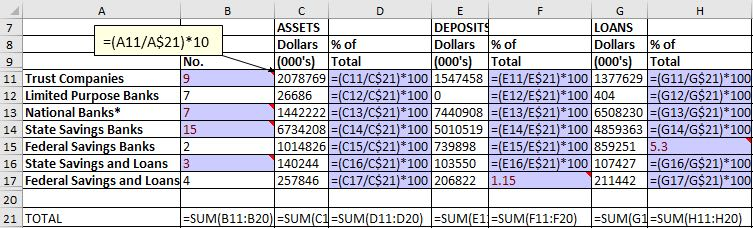
\includegraphics[width=\columnwidth]{figure/figure2.png}
    \caption{用于展现\wa 的单个单元格有效性精化方法的工作表``Summary1201''。\cu 检测出一个单元格类(用紫色标记),导致四个误报的缺陷(用红色三角标注),不过这四个单元格会被\wa 的单个单元格有效性精化方法排除出去,也就不再被错误标记为缺陷。}
    \label{figure2}
\end{figure}
第一个精化方法考虑的是,当 \wa 用额外的数值单元格扩充种子类时,这类被扩充进来的单元格自身是否是有效的(有效指适合加入到)。
但在实际情况下,并没有直接的方法判断这类数值单元格是否有效,换言之,是否应该被扩充,因为它们仅包含纯数值,从它自身出发看,和其他单元格没有任何可见的计算关系。
不过,因为这些被扩充的单元格和种子类中的原始单元格即将被合并为同类,那么根据单元格类的定义,它们应该享有一个共同的计算目标。
那么,这些被扩充的单元格的值应当可以和原始单元格相同的公式计算出来。
为了验证这一预期,\wa 会测试种子类中单元格具有的所有公式,来判断是否至少存在一个公式的计算结果和被扩充的这个单元格的值保持一致。
具体而言,当我们用一个公式来替换当前数值单元格里的内容时,该单元格应该是可计算的。
否则,如果所有公式的测试都以失败告终(例如引用一个错误的单元格内容或者无效的单元格引用),这个被扩充的数值单元格就是有问题的,进而应当被阻止扩充进该类。
这种方法就被称为\textit{单个单元格的有效性精化}。
% 这里可以解释一下什么是 “用公式替换数值” 的思路

如图\ref{figure2}所示,工作表“Summary1201”给出了一个案例,其中 25 个单元格(B11,B13,B14,B16,D11-17,F11-17和 H11-17)被\cu 划分为同类(用紫色标注)。
\cu 检测出了 6 个缺陷(用红色三角标注),其中 2 个(F17 和 H15)是真阳性,另外四个(B11,B13,B14 和 B16)是假阳性。后四个数值单元格被扩充进这个类,是因为它们具有和种子类中起始的单元格类似的弱特征(例如相似的表头和布局)。
然而,根据\wa 的单个单元格有效性精化方法,这样的扩充是有问题的。
事实上,如果这四个单元格中的任意一个被扩充到这个类中,这个单元格把它的值和任意一个类中包含的公式计算出来的值相一致。
例如,考虑单元格 B11,按照类中包含的公式来看,对于它来说最好的潜在公式应该是“=(A11/A\$21)*100”。
然而,这个公式是不可计算的,因为单元格 A11 和 A\$21指向字符串单元格,无法参与这类除法算数运算中。
相似的问题也出现在单元格 B13,B14 和 B16。 
因此,\wa 会防止这类数值单元格被扩充到类中。


\section{多个单元格之间的有效性精化方法}
\begin{figure}[tbp]
    \centering
    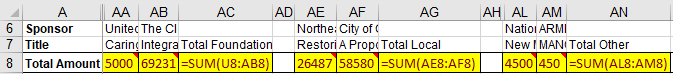
\includegraphics[width=\columnwidth]{figure/figure3.png}
    \caption{用于展现\wa 的多个单元格有效性精化方法的工作表``Detail for the College of A\&S''。\cu 检测出一个单元格类(用黄色标记),并进而导致六个假阳性的缺陷被报告出来(用红色三角形标注),不过这六个单元格会被\wa 的多单元格有效性精化方法从类中排除出去,进而不会再被错误的标记为有缺陷的单元格。}
    \label{figure3}
\end{figure}
第二个精化方法考虑的是,当 \wa 用额外的数值单元格扩充种子类时,这类被扩充进来的单元格不会破坏种子类中已有单元格之间的属性。
我们拿单元格的引用举例,因为这是电子表格单元格的重要特征。
假设种子类中已有单元格的引用从不会彼此重叠,那么我们会预期一个被扩充进来的数值单元格当它被加入到这个类中,并且它的值被类中某个其他单元格的公式替换时,也不会违反这个属性。
这个预期也可以以一种相反的方式表达出来,即一个单元格类中的已有公式之间的引用已经彼此重叠了,那么对于被新扩充进来的数值单元格也不能发生不相交的情况。
也就是说,这个属性应当对类中所有的单元格保持一致(不管是原有的单元格,还是被扩充进来的单元格),这可以被看作电子表格中标的编辑风格。
另外,如果检测到违反该一致性的数值单元格,它就应当被禁止扩充到这个类中。
这种方法就被成为\textit{多个单元格的有效性精化}。

如图\ref{figure3}所示,工作表“Detail for the College of A\&S” 给出了一个案例。
其中,9 个单元格(AA8, AB8, AC8, AE8, AF8, AG8, AL8, AM8和AN8)被\cu 划分到同一个类中(用黄色标记)。
接着,\cu 检测出 6 个单元格缺陷(AA8, AB8, AE8,AF8,AL8和AM8),因为它们只包含纯数值,但这六个缺陷都是假阳性。
不过,\wa 能够禁止这六个单元格(AA8, AB8, AE8,AF8,AL8和AM8)被扩充进来,从而避免了这六个误报的情况。
事实上,这六个数值单元格并不和其他三个公式单元格(AC8,AG8和AN8)共享相同的计算目标。
前面的数值单元格代表了用户直接给出的具体的数值,而另外三个公式则是计算它们各自左侧的若干个单元格的和。
\wa 通过它的多个单元格有效性精化方法区分出这两类:后三个公式单元格的引用范围是互不重叠的,但如果把前面 6 个数值单元格扩充进来,并用任意一个公式来替换它们的值,这个属性会遭到破坏。
例如,当把单元格 AF8 中的数值用单元格 AG8 里的公式模板替换成公式“=SUM(AD8:AE8)”时,它的引用单元格(AD8 和 AE8)会和单元格 AG8 的引用单元格(AE8 和 AF8)发生重叠。
相似的问题也会出现在单元格 AA8,AB8,AE8,AL8 和 AM8 上。
因此,\wa 会禁止这类数值单元格被扩充到类中。


\section{针对整个类的有效性精化方法}
\begin{figure}[tp]
    \centering
    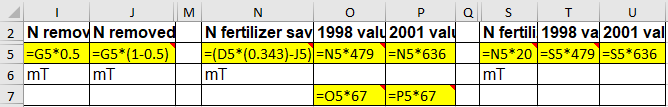
\includegraphics[width=\columnwidth]{figure/figure4.png}
    \caption{用于展现\wa 的整个类有效性检验方法的工作表``World 1996''。\cu 识别出了一个类(用花色标记出来,但整个类是不合理的),进而导致所有相关的单元格都被错误地标记为有缺陷的(用红色三角形标记),不过这个类会被\wa 的整个类的有效性检验方法移除掉,进而相关的所有单元格也不会被错误地标记为有缺陷的。}
    \label{figure4}
\end{figure}
最后一种精化方法考虑的是最终形成单元格类的整体有效性,即它关注于类层面而不是单元格层面的有效性属性。
我们预期在这个类中应该存在一个统一的公式能够覆盖大多数单元格,也就是说大多数单元格应当遵循一个共同的计算目标。
\wa 会测试类中所有现存可获得的公式,如果没有任何一个能够满足这个目的,\wa 就会认定这个类为不合格的,并将该类从所有类的集合中删除,以避免后续在缺陷检测过程中将绝大多数单元格标记为有缺陷的,即产生大量误报。
这种方法就被称为\textit{整个类的有效性精化方法}。

如图\ref{figure4}所示,工作表“World 1996”给出了一个案例。
其中,\cu 把 10 个单元格划分为同一个类(用黄色标注)。
进而 \cu 把其中的 7 个检测为有缺陷的单元格,但这 7 个都是假阳性。
事实上,这10 个单元格包含几乎完全不同的公式(5 种计算模式),这强烈地表明它们本质上遵循不同的计算目标。
通过我们的类级别的有效性精化方法,\wa 会将该类完整地从类集合中删除。
这里需要注意的是,\wa 需要一个阈值来控制“覆盖大多数单元格”这个判断的程度。
安全起见,\wa 选择一个保守的值,即 50\%,来尽可能保护单元格类不被排除在外(作为对比,\ca 选择了相对激进的值70\%)。


\section{有效性校验方法的执行过程}
根据它们之间的依赖关系,\wa 将这三个基于有效性精化属性的方法依次应用在单元格聚类之后。
它们彼此互补,并且由下而上地在不同层面起作用(从单个单元格内部,到多个单元格之间,最后再到整个类的有效性上)。
它们的目标是共同提升单元格聚类有效性,使得聚类结果更加具有稳定和可靠,最终对缺陷检测阶段起到积极作用,极大地减少缺陷误报率,这部分也会在第六章的实验评估部分进行验证。